\section{Layered architecture and smart UI overview}\label{sec:01}
    Layered architecture is a great concept, well described in the book «Domain Driven Design» by Eric Evans. This is a very good concept for separation of concerns. In this essay I would like to share my thoughts on this approach from my experience as an iOS software engineer. So Eric Evans describes four layers of a software solution: UI, Application layer, Domain layer and Infrastructure layer. Each of this layers has its own purpose and responsibility, which helps us not only to separate concerns, but to easily change some parts of a software(chage database, because it is connected via interface etc.) and reuse existing(use iOS`s Application, Domain and Infrastructure layers to connect to MacOS`s, WatchOS, tvOS UI etc.). But as Eric Evans  describes some great advantages and disadvantages of it, which I mostly agree, might be a stopper some teams. The most important disadvantage, in my opinion, is it is very difficult to work with layered architecture for a team of inexperienced developers and we have to spend some time digging deep into this topic in order to make software development process smooth and easy. 

	And what about smart UI? Actually Eric Evans explained a really good point, and even better to say mindset of any developer who is willing to implement this pattern. «Put all business logic into the user interface. hop the application into small functions and implement them as a separate user interfaces, embedding the business rules into them. Use a relational database as a shared repository of data. Use the most automated UI building and visual tools available». And this is exactly one of the most common problems with modern MVC implementation. In the next chapter I would like to explain why Apple`s MVC is a smart UI, and what problems  and confusions regular developers face trying to separate concerns simply using MVC in iOS applications.
\section{Overview of Apple`s MVC architecture in iOS}\label{sec:02}
When you start developing iOS applications, first tutorials that you will see will belong to Apple. You read all their fancy documentation, gets excited with Swift`s syntax sugar and finally start building you first app. On their website( https://developer.apple.com/library/archive/documentation/General/Conceptual/DevPedia-CocoaCore/MVC.html ) they suggest to you to use MVC, describing the responsibility of every module and connection between them.
	\begin{figure}[!htbp]
	\centering
	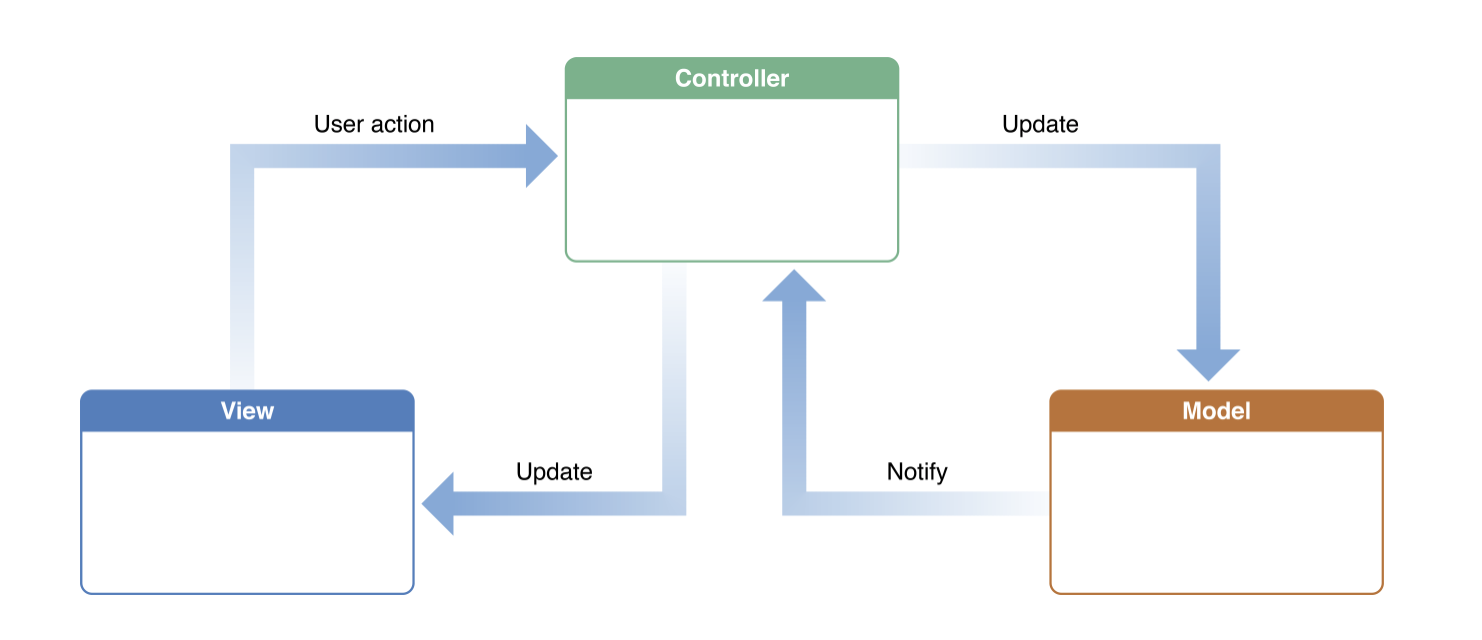
\includegraphics[width=0.95\linewidth]{sections/01-chapter/images/Controller.png}
	\caption{MVC on Apple Website.}\label{sec:01_01:fig:01}
	\end{figure}
But the main problems appears when you are trying to implement it in your first app. But first I have to describe the peculiarity of iOS development. There are two approaches of building the UI layer available today: imperative and declarative. There are no problems with declarative approach, it is available using newly presented ui framework called SwiftUI, it forbids for developers to include any business logic into UI layer by design, but is is available for developer for a year now. This framework is on early stage of beta-testing, so it is not really useful for real-life development. But we are going to look at the most popular framework, which imperative called UIKit. To prove its popularity lets check the reversed-engineered code of the latest iOS 14 https://apptractor.ru/info/articles/kakie-jazyki-programmirovanija-ispolzujutsja-vnutri-ios-14.html and SwiftUI is less than 1 percent of overall code. So with UIKit there are two main approaches of building UI - visually via XML file and from code via Swift. Apple provides us with starting base class called UIViewController, which is responsible for holding UI object with strong reference and process user gestures and actions(swipes, button touches etc.). Junior developers love to build UI from XML, sometimes is very useful and very easy to understand for new developers, because they do not have to read UI from code and imagine how it looks like on device.  So we are going to see how this approach works. You have your UI built in XML file and some its views connected to UIViewController class using @IBOutlet and @IBActions decorators. And your UIViewController class is not fully a view, since you have your view built in xml, and fully a controller, because it has some UI views and user actions connected. At this point your UIViewController becomes smart UI, where you handle user gestures, change UI and store business logic. Furthermore, iOS SDK gives you very useful decorators to easily use persistence storage - SQLite Database. So not only UIViewController combines UI layer, Domain layer and Infrastructure layer, but also handles navigation logic, dependency injection etc., so responsibility of Application layer is also on UIViewController. There is a huge temptation to use smart UI like this for small projects, but very often your UIViewController exceeds 800 lines, than 1000 lines, and at some project I have seen 5000 lines UIViewController. 

